\documentclass[11pt]{article}
\usepackage[letterpaper]{geometry}
\usepackage{MATH561}
\usepackage{SetTheory}

\begin{document}
\noindent \textbf{\Large{Caleb Logemann \\
MATH 561 Numerical Analysis I \\
Homework 2
}}

\begin{enumerate}
    \item
        \begin{enumerate}
            \item[(a)] \hfill \\
                \begin{center}
                    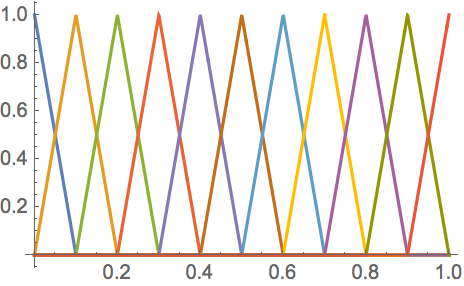
\includegraphics[scale=.5]{Figures/02_1a.png}
                \end{center}

            \item[(b)]
                If $j = k$, then $\pi_j\p{k/n} = \pi_j{j/n} = 1$.
                If $j \neq k$, then $\pi_j\p{k/n} = 0$, because $k/n$ is
                outside of the division that is the support of $\pi_j$

            \item[(c)]
                Let $c_0, c_1, \ldots, c_n \in \RR$ be given such that
                $\sum{i=0}{n}{c_i \pi_i\p{t}} = 0$ for all $t \in \p{0,1}$
                Consider $t = k/n$ for some $k \in \set{0, 1, \ldots, n}$, then
                $\sum{i=0}{n}{c_i \pi_i\p{k/n}} = c_k \pi_k\p{k/n}$, because
                $\pi_j{k/n} = 0$ for all $j \neq k$.
                Also $\pi_k\p{k/n} = 1$, so $c_k \pi_k\p{k/n} = c_k$.
                However this sum must be equal to $0$ at $t = k/n$, so $c_k = 0$.
                This implies that $c_0 = c_1 = \cdots = c_n = 0$.
                Thus the $\set{\pi_j}_{j=0}^n$ is linearly independent over the
                interval $(0, 1)$.
                This also implies that $\set{\pi_j}_{j=0}^n$ is linearly independent 
                over the points $\set{0, 1/n, \ldots, \frac{n-1}{n}, 1}$, because
                at these points only one of the functions contributes to the
                overall sum.

            \item[(d)]
                For $\abs{i - j} > 1$, $\pi_i(t) \pi_j(t) = 0$ for $t \in (0, 1)$.
                Therefore $\dintt{0}{1}{\pi_i(t) \pi_j(t)}{t} = 0$ and $a_{ij} = 0$
                for $\abs{i - j} > 1$.

                For $\abs{i - j} = 1$, without loss of generality assume $j = i + 1$.
                Note that $\supp\p{\pi_i(t)\pi_j(t)} = (i/n, i+1/n) = (i/n, j/n)$
                \begin{align*}
                    \dintt{0}{1}{\pi_i(t)\pi_j(t)}{t} &= \dintt{0}{1}{\pi_i(t)\pi_{i+1}(t)}{t}
                    \intertext{Since $\supp\p{\pi_i(t)\pi_{i+1}(t)} = (i/n, i+1/n)$}
                    &= \dintt{i/n}{\p{i+1}/n}{\pi_i(t)\pi_{i+1}(t)}{t}
                    \intertext{On this interval $\pi_i(t) = -nt + i + 1$ and $\pi_{i+1}(t) = nt - i$}
                    &= \dintt{i/n}{\p{i+1}/n}{\p{-nt + i + 1}\p{nt - i}}{t} \\
                    &= \dintt{i/n}{\p{i+1}/n}{-n^2t^2 + int + int + nt - i^2 - i}{t} \\
                    &= \dintt{i/n}{\p{i+1}/n}{-n^2t^2 + (2i+1)nt - i^2 - i}{t} \\
                    &= \eval{-\frac{n^2}{3}t^3 + \frac{(2i+1)n}{2}t^2 - (i^2 + i)t}{t=i/n}{\p{i+1}/n} \\
                    &= \eval{-\frac{n^2}{3}t^3 + \frac{(2i+1)n}{2}t^2 - (i^2 + i)t}{t=i/n}{\p{i+1}/n} \\
                    &= -\frac{n^2}{3}\p{\frac{i+1}{n}}^3 + \frac{(2i+1)n}{2}\p{\frac{i+1}{n}}^2 - (i^2 + i)\frac{i+1}{n} +
                    \frac{n^2}{3}\p{\frac{i+1}{n}}^3 - \frac{(2i+1)n}{2}\p{\frac{i}{n}}^2 + (i^2 + i)\frac{i}{n} \\
                    &= 
                \end{align*}

        \end{enumerate}

    \item % #2 finding upper bounds for error
        \begin{enumerate}
            \item[(a)]
                
            \item[(b)]
        \end{enumerate}

    \item % #3
    \item % #4
    \item % #5
    \item % #6
        \begin{enumerate}
            \item[(a)]

            \item[(b)]
                \begin{enumerate}
                    \item[(b.1)]
                    \item[(b.2)]
                    \item[(b.3)]
                \end{enumerate}
        \end{enumerate}

    \item % #7
    \item % #8
\end{enumerate}
\end{document}
